\documentclass[conference]{IEEEtran}
\IEEEoverridecommandlockouts
\usepackage{cite}
\usepackage{amsmath,amssymb,amsfonts}
\usepackage{algorithmic}
\usepackage{graphicx}
\usepackage{textcomp}
\usepackage{xcolor}
\usepackage{multirow}
\def\BibTeX{{\rm B\kern-.05em{\sc i\kern-.025em b}\kern-.08em
    T\kern-.1667em\lower.7ex\hbox{E}\kern-.125emX}}
\begin{document}

\title{Smart Spreading Factor Assignment for LoRaWANs}


\author{\IEEEauthorblockN{Tugrul Yatagan and Sema Oktug}
\IEEEauthorblockA{Department of Computer Engineering,
Istanbul Technical University\\
Istanbul, Turkey\\
Email: \{yatagan, oktug\}@itu.edu.tr}}
\maketitle


\begin{abstract}
Low power wide area network (LPWAN) technologies offer affordable connectivity to massive number of low-power devices distributed over large geographical areas. Focus of this work is one of the most promising LPWAN technologies: LoRa. LoRa offers long range communication and strong resilience to interference by proprietary modulation technique based on Chirp Spread Spectrum (CSS). LoRa modulation trades data rate for sensitivity and communication range by spreading symbols within a fixed channel bandwidth. Collisions in LoRaWAN networks are strongly related with spreading factor (SF) assignment of nodes which indeed effects network performance. In this work, a simulation environment to evaluate the performance of SF assignment schemes is implemented. Furthermore, a novel smart SF assignment strategy which utilizes Support Vector Machine (SVM) and Decision Tree Classifier (DTC) machine learning techniques for optimization of SF assignment is proposed. It is observed and presented that the proposed smart SF assignment techniques give promising simulation results in terms of packet delivery ratio (PDR).
\end{abstract}


\begin{IEEEkeywords}
LoRa, LoRaWAN, Spreading Factor, LPWAN, Machine Learning
\end{IEEEkeywords}


\section{Introduction}
\IEEEPARstart{N}{umber} of Internet of Things (IoT) applications increased exponentially in last few years \cite{7721743}. Recent developments on LPWAN technologies has great impact on growth of number of IoT applications. LPWAN technologies address some of the well-known wireless communication challenges. Traditional wireless communication methods such as cellular networks (e.g., 2G, 3G, LTE) and short-range communication technologies (e.g., Bluetooth, WiFi, Zigbee) cannot provide low power and long range at the same time. Cellular networks can provide long range and high data rate, but they are complex and consume too much power. Besides, most of the IoT applications do not require high data rate. Short-range communication methods can provide relatively low power consumption, but their range is limited to a few hundred meters at best \cite{7815384}. LPWAN technologies fill the technology gap between short range and cellular technologies by providing low power and long-range communication. LPWAN technologies basically sacrifice data rate to provide low power consumption.

There are several emerging LPWAN technologies. LoRa, Sigfox, NB-IoT and LTE-M are commonly used, well-known LPWAN technologies \cite{7815384}. LoRa and Sigfox use license free ISM frequency bands while NB-IoT and LTE-M use licensed frequency bands which brings extra cost \cite{7815384}. Both LoRa and Sigfox are known for ultra-low power consumption and resilience to interference. While NB-IoT and LTE-M are promoted for higher data rate. LoRa has open standard MAC protocol called LoRaWAN. LoRaWAN and Sigfox MAC protocols are based on pure ALOHA medium access. LoRaWAN networks can be deployed as a private network like WiFi. However, Sigfox and NB-IoT are only available with operator contract \cite{7815384}.

LoRa can adjust data rate by spreading symbols within a fixed channel bandwidth. This enables tradeoff between receive sensitivity and air time of transmission \cite{7803607}. Simultaneous same SF transmissions are prone to collision, however, different SF transmissions in the same channel are orthogonal to each other. Thus, SF assignment is crucial for overall network performance. In this work, a LoRa discrete event simulator is developed to study the performance of LoRa SF assignment strategies. Also, a machine learning based SF assignment approach is proposed. Support Vector Machine (SVM) and Decision Tree Classifier (DTC) techniques are employed and the introduced schemes are called as smart SF schemes. The performance of the smart schemes are compared with the performance of the lowest SF assignment scheme. It is shown that the proposed smart SF assignment schemes give promising results.

This paper is organized as follows: Section \ref{LoRa} and Section \ref{LoRaWAN} provides some background information about LoRa and LoRaWAN. Section \ref{Related Works} summarize  the other related works. Section \ref{Proposed Technique} describes the smart SF assignment technique proposed. Simulation environments and results are shown in Section \ref{Simulation Environment} and \ref{Simulation Results}. Finally, Section \ref{Conclusion} concludes the paper by giving future directions.


\section{LoRa} \label{LoRa}
LoRa is a proprietary physical layer radio/chipset technology that provides wireless link solution for low power wide area networks. It uses proprietary spread spectrum modulation technique that is the derivative of Chirp Spread Spectrum (CSS). A chirp is a sinusoidal signal of which frequency increases over time. Chirp frequency increases linearly and sweeps the entire bandwidth \cite{AN1200.22}.

\subsection{Spreading Factor}
The ratio between symbol and chirp rate is equal to $2$\textsuperscript{SF}. SF can take values between 7 to 12. SF also determines data rate of a LoRa transmission \cite{AN1200.22}. Data rate of a LoRa transmission can be calculated as:

\begin{equation} \label{eq:bit_rate_sf}
R_{b} = SF * \dfrac{\left[ \dfrac{4}{4+CR} \right] }{ \left[ \dfrac{2^{SF}}{BW|_{Hz}} \right]} \ bps
\end{equation}

Where, $R_{b}$ is data rate in bps, SF is spreading factor $SF \in \{7,..,12\}$, CR is error correction code rate $CR \in \{1,..,4\}$ and $BW$ is bandwidth in Hertz \cite{AN1200.22}.

When BW and CR are constant, as the SF increases, the data rate decreases. Increasing the SF makes the signal more resilient to noise thus increases the transmission range. Increasing the SF also increases the transmission duration which increases the power consumption. Therefore, it is possible to trade between range and power consumption by changing SF.

\subsection{Spreading Factor Assignment Issue}
Simultaneous different SF transmissions are orthogonal to each other up to some extent. Which means that, a LoRa gateway can simultaneously receive multiple transmissions with different SFs. However, simultaneous transmissions with the same SF may not be received by the gateway due to collision. For this reason, SF assignment of nodes is crucial for network performance.

In a LoRaWAN network, initially, a node is not aware of how far away it is from a gateway. However, a node can guess the distance from a gateway by observing received signal power of a downlink transmission. If received signal power of a downlink transmission is too high, then node can decrease its next transmission SF to decrease power consumption. This SF assignment method is called lowest possible SF assignment scheme for the rest of the paper. Lowest possible SF assignment scheme is commonly used in LoRaWAN deployments. Also, a gateway can request from a node to decrease its SF or transmit power.

In Figure \ref{fig:collision}, a LoRaWAN network deployed with a single gateway is illustrated. Different color rings represent achievable range of different SFs from the gateway and different color circles represent selected SF of the nodes. The end devices close to the gateway will fall into the lowest SF (SF7) area section. The end devices close to the gateway will probably select the lowest SF most of the time. This causes a lot of collisions between same SF transmissions. Hence the number of collisions will increase as the number of end devices close to the gateway increases.

\begin{figure}
\centering
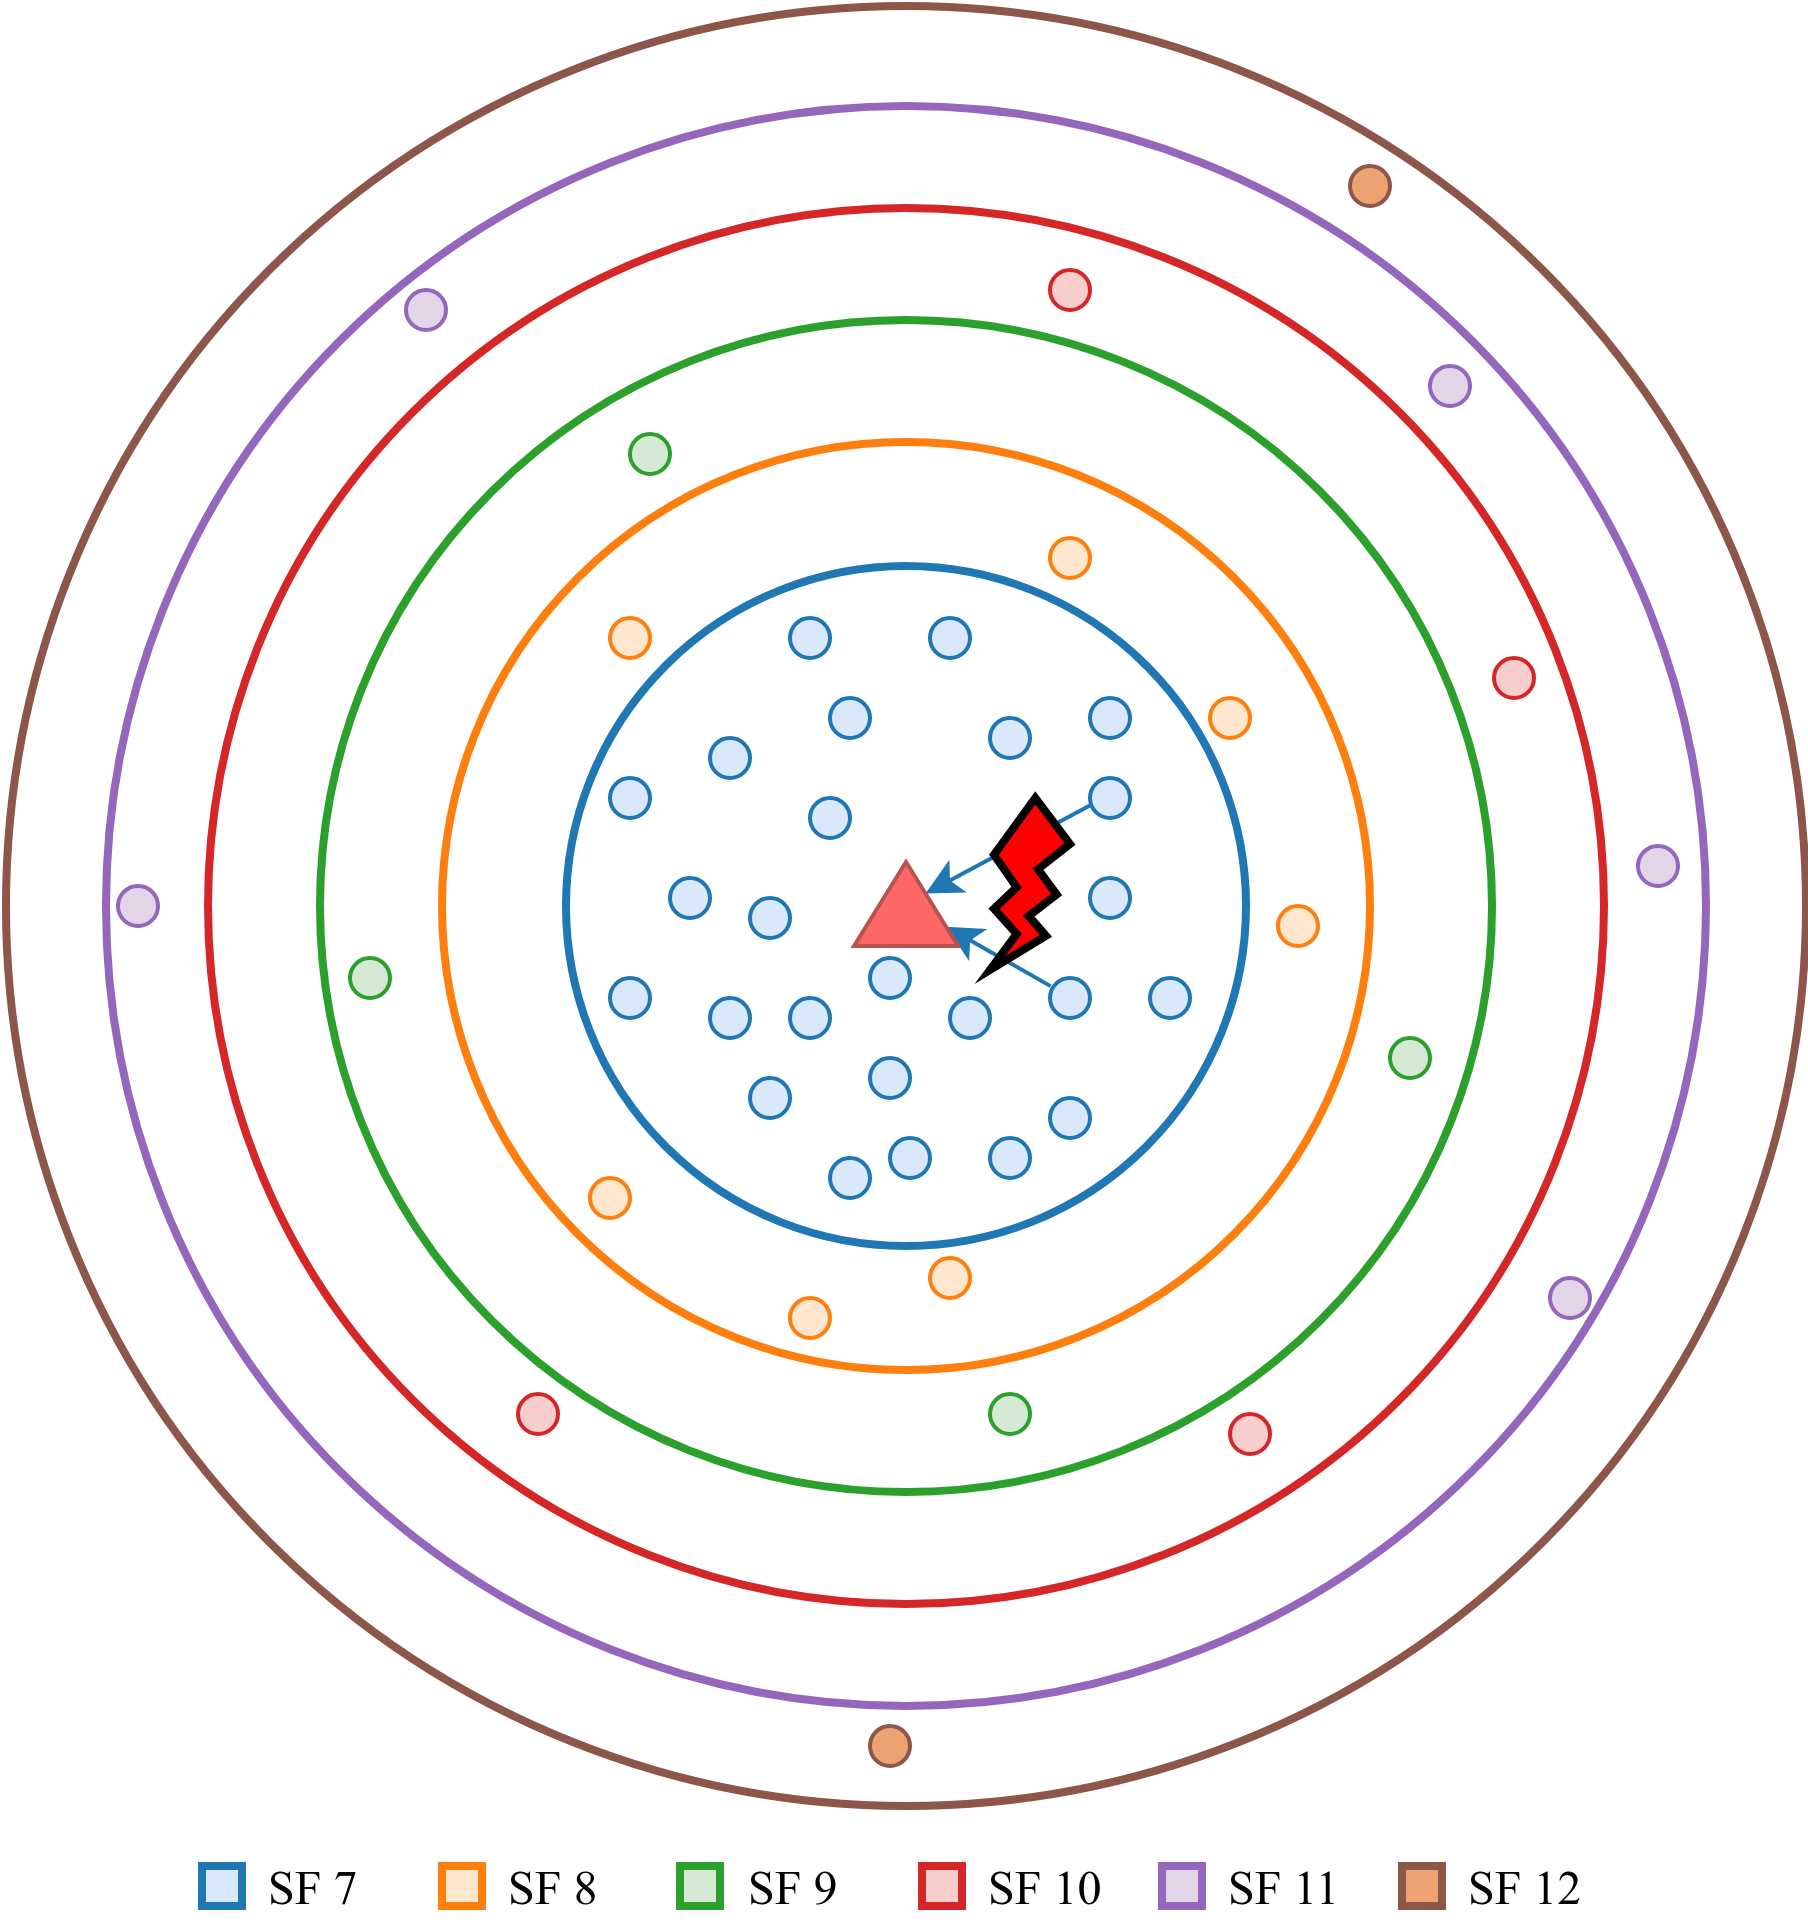
\includegraphics[width=0.85\linewidth]{collision.png}
\caption{Collision between nodes close to the gateway.}
\label{fig:collision}
\end{figure}


\section{LoRaWAN} \label{LoRaWAN}
LoRa has an open standard medium access control (MAC) layer protocol called LoRaWAN which is designed for large scale LoRa networks considering well known LPWAN challenges and their best practice solutions. LoRaWAN is developed and maintained by LoRa Alliance. LoRa Alliance is an open, non-profit organization dedicated to standardization of LoRaWAN. LoRaWAN provides inter-operability between different LoRa networks. LoRa can be used as a wireless link technology without complying LoRaWAN, however this would break inter-operability between different LoRa networks. LoRaWAN is based on pure ALOHA medium access which means that end nodes do not check whether the channel is free or not before transmission, accepting the possibility of a collision. A typical LoRaWAN network consists of following three network entities.

\subsection{End node}
LoRaWAN end node (EN) is a low power embedded device that only communicates to gateways. LoRaWAN standard defines three classes for end devices which are Class A, Class B, and Class C. Different classes provide LPWAN solutions to different applications and deployments. Class A end nodes generate uplink transmission at any time and only receive a period of time after uplink transmission. Class B end nodes extend Class A behavior by adding scheduled receive windows for downlink transmission. Receive window is synchronized using a beacon packet transmitted by gateways. Class C end nodes extend Class A behavior by keeping receive window open all the time except uplink transmission. This provides Class C end nodes with low latency downlink communication, which requires more power consumption. In this paper, only Class A end devices are considered since Class A behavior leads to the lowest power consumption.

\subsection{Gateway}
LoRaWAN gateway (GW) is a device that receive/transmit packets coming from/to end nodes. A typical gateway can receive from multiple channels at the same time. Gateways are usually connected to power grid, so power consumption of a gateway is insignificant in most of the deployments.

\subsection{Network server}
LoRaWAN network server (NS) is a server that provides MAC layer processing. Network server routes messages from application to end nodes and vice versa. Network server can be used for tweaking end node parameters like channel, transmit power and SF to increase network performance.


\section{Related Works} \label{Related Works}
The literature related to the work presented in this paper has started to grow recently. LPWAN technologies and especially LoRa attracted researchers’ attentions lately. Some of these works which studies LoRa/LoRaWAN SF are summarized.

In \cite{7996384}, the authors evaluated the performance of LoRaWAN networks in a smart city scenario. The authors proposed a link measurement and a link performance model for LoRa. The authors also proposed a SINR threshold matrix for modeling LoRa interference between simultaneous but different SF LoRa transmissions. They implemented a LoRa simulator in ns-3 to study scalability and performance of LoRaWAN networks. Their results show that SF assignment has great effect on LoRaWAN network performance.

In \cite{8090518}, another LoRaWAN ns-3 simulator is presented. Authors introduced an error model for determining range as well as interference between multiple simultaneous LoRa transmissions. Their simulator supports LoRaWAN Class A end devices, multiple gateways, both upstream and downstream confirmed messages. Their results show that allocating network parameters such as SF is highly important for the performance of LoRaWAN networks.

In \cite{8267219}, the authors studied the effects of imperfect orthogonality between different LoRa SF transmissions. The authors state that a LoRa transmission can be interfered by a different SF transmission when power of the interfering signal is significantly greater than the reference signal. Their experimental results show that this power difference is around 16 dB. Such a power difference can be seen when an interfering signal is close to a receiver or the sum of interfering signals' energy can create this power difference.

\par In \cite{8267219} and \cite{8430542}, the authors studied the effects of imperfect orthogonality between different LoRa SF transmissions. The authors state that a LoRa transmission can be interfered by a different SF transmission when power of the interfering signal is significantly greater than the reference signal. Their results show that transmission among different SFs can cause a significant impact in high-density LoRaWAN networks.

The adaptive data rate (ADR) algorithm recommended by Semtech Corporation utilizes signal to noise ratio (SNR) of the last 20 transmissions to minimize the transmit power and SF while ensuring successful transmissions \cite{lorawan_adr}. The recommended algorithm uses a predefined SF and corresponding required SNR table. The algorithm considers maximum SNR of the last 20 transmissions. The algorithm increases transmit power or decrease data rate in case of low SNR and the opposite in case of high SNR.


\section{Proposed Technique} \label{Proposed Technique}
The collision problem illustrated in Figure \ref{fig:collision} is solved by forcing some of the close nodes to select higher SFs even though they are able to communicate with lower SFs. This has potential to prevent collisions due to the orthogonality of the SFs as shown in Figure \ref{fig:collision_solution_single_gw}. Higher SF assigned nodes are drawn with bold circle border in Figure \ref{fig:collision_solution_single_gw}. However, distribution of SF among nodes becomes an important problem. Increasing a node's SF should be done carefully since higher SF means longer air time and longer air time means increasing the probability of collisions with other high SF transmissions. In multiple gateways scenarios, this approach may increase the collisions with the nodes in other gateway's range. Thus, extra care should be taken for nodes in the intersection area of the gateways illustrated in Figure \ref{fig:collision_solution_multi_gw}.

It is difficult to propose a single SF assignment rule for every possible LoRaWAN topology since every network is different and optimizing their nodes' SFs requires different rules. For this reason, machine learning based SF assignment approach is proposed to decrease the collisions for the same SF transmissions. This technique starts by learning the transmission behavior of the nodes in a network. An NS can keep track of successful uplink transmissions and their SFs. This NS can also keep track of some of the collided transmissions if header part of the packet is not interfered at the gateway. However, NS cannot keep track of transmissions with lower receive power than sensitivity of the gateway. Using those obtained information, NS can train a classifier to predict future transmission result for a specific node and a specific SF. Using this prediction model NS can assign SFs to nodes considering the collision probability.

In this work, decision tree classifier (DTC) and support vector machine (SVM) \cite{Alpaydin} schemes are employed to predict the transmission results. Class weights are balanced according to sample distributions for both methods. For DTC, Gini impurity criteria is used to measure the quality of splits. For SVM, penalty parameter is set to 1, degree is set to 3 and RBF kernel is used.

It is possible to generate mass amount of LoRaWAN transmission logs for different topologies using our simulator. Training dataset size is directly proportional to simulation duration. Thus, increasing the simulation duration, improves the prediction accuracy up to some extent. In real world deployments, NS can keep track of transmissions and it can create a classifier daily basis, then gateways can request from nodes to use suggested SFs.

There are three features in the dataset generated by the simulation tool. Features of the dataset are: X coordinate of the transmission source, Y coordinate of the transmission source and SF of the transmission. X and Y coordinate feature values are continuous numbers. SF feature values are integer numbers between 7 to 12. Class label of the dataset is the result of the transmission. Class label values are successful, interfered and under sensitivity. DTC and SVM prediction schemes are integrated into the simulation tool to study smart SF assignment schemes. A classifier is trained from generated dataset and this classifier is used for selecting optimum SF for the nodes in the network.

The tool first runs a simulation with random SF scheme. After random SF scheme simulation completed, transmission logs are combined into three feature columns and one class label column to create the training dataset. Then the dataset is fed to Python scikit-learn DTC or SVM classifiers for training phase. After the classifier model is built, second simulation is run with the trained classifier. The tool selects optimum SF for transmissions considering prediction of the transmissions. For every transmission, the classifier predicts the transmission result for the lowest possible SF. If the transmission result is predicted as interfered, then the tool increases the SF and predicts a new transmission result. If the new transmission result is classified as successful, then simulator continue to execute with selected SF. If no SF transmission result is predicted as successful, then the tool selects the lowest possible SF and continue to execute.

\begin{figure}
\centering
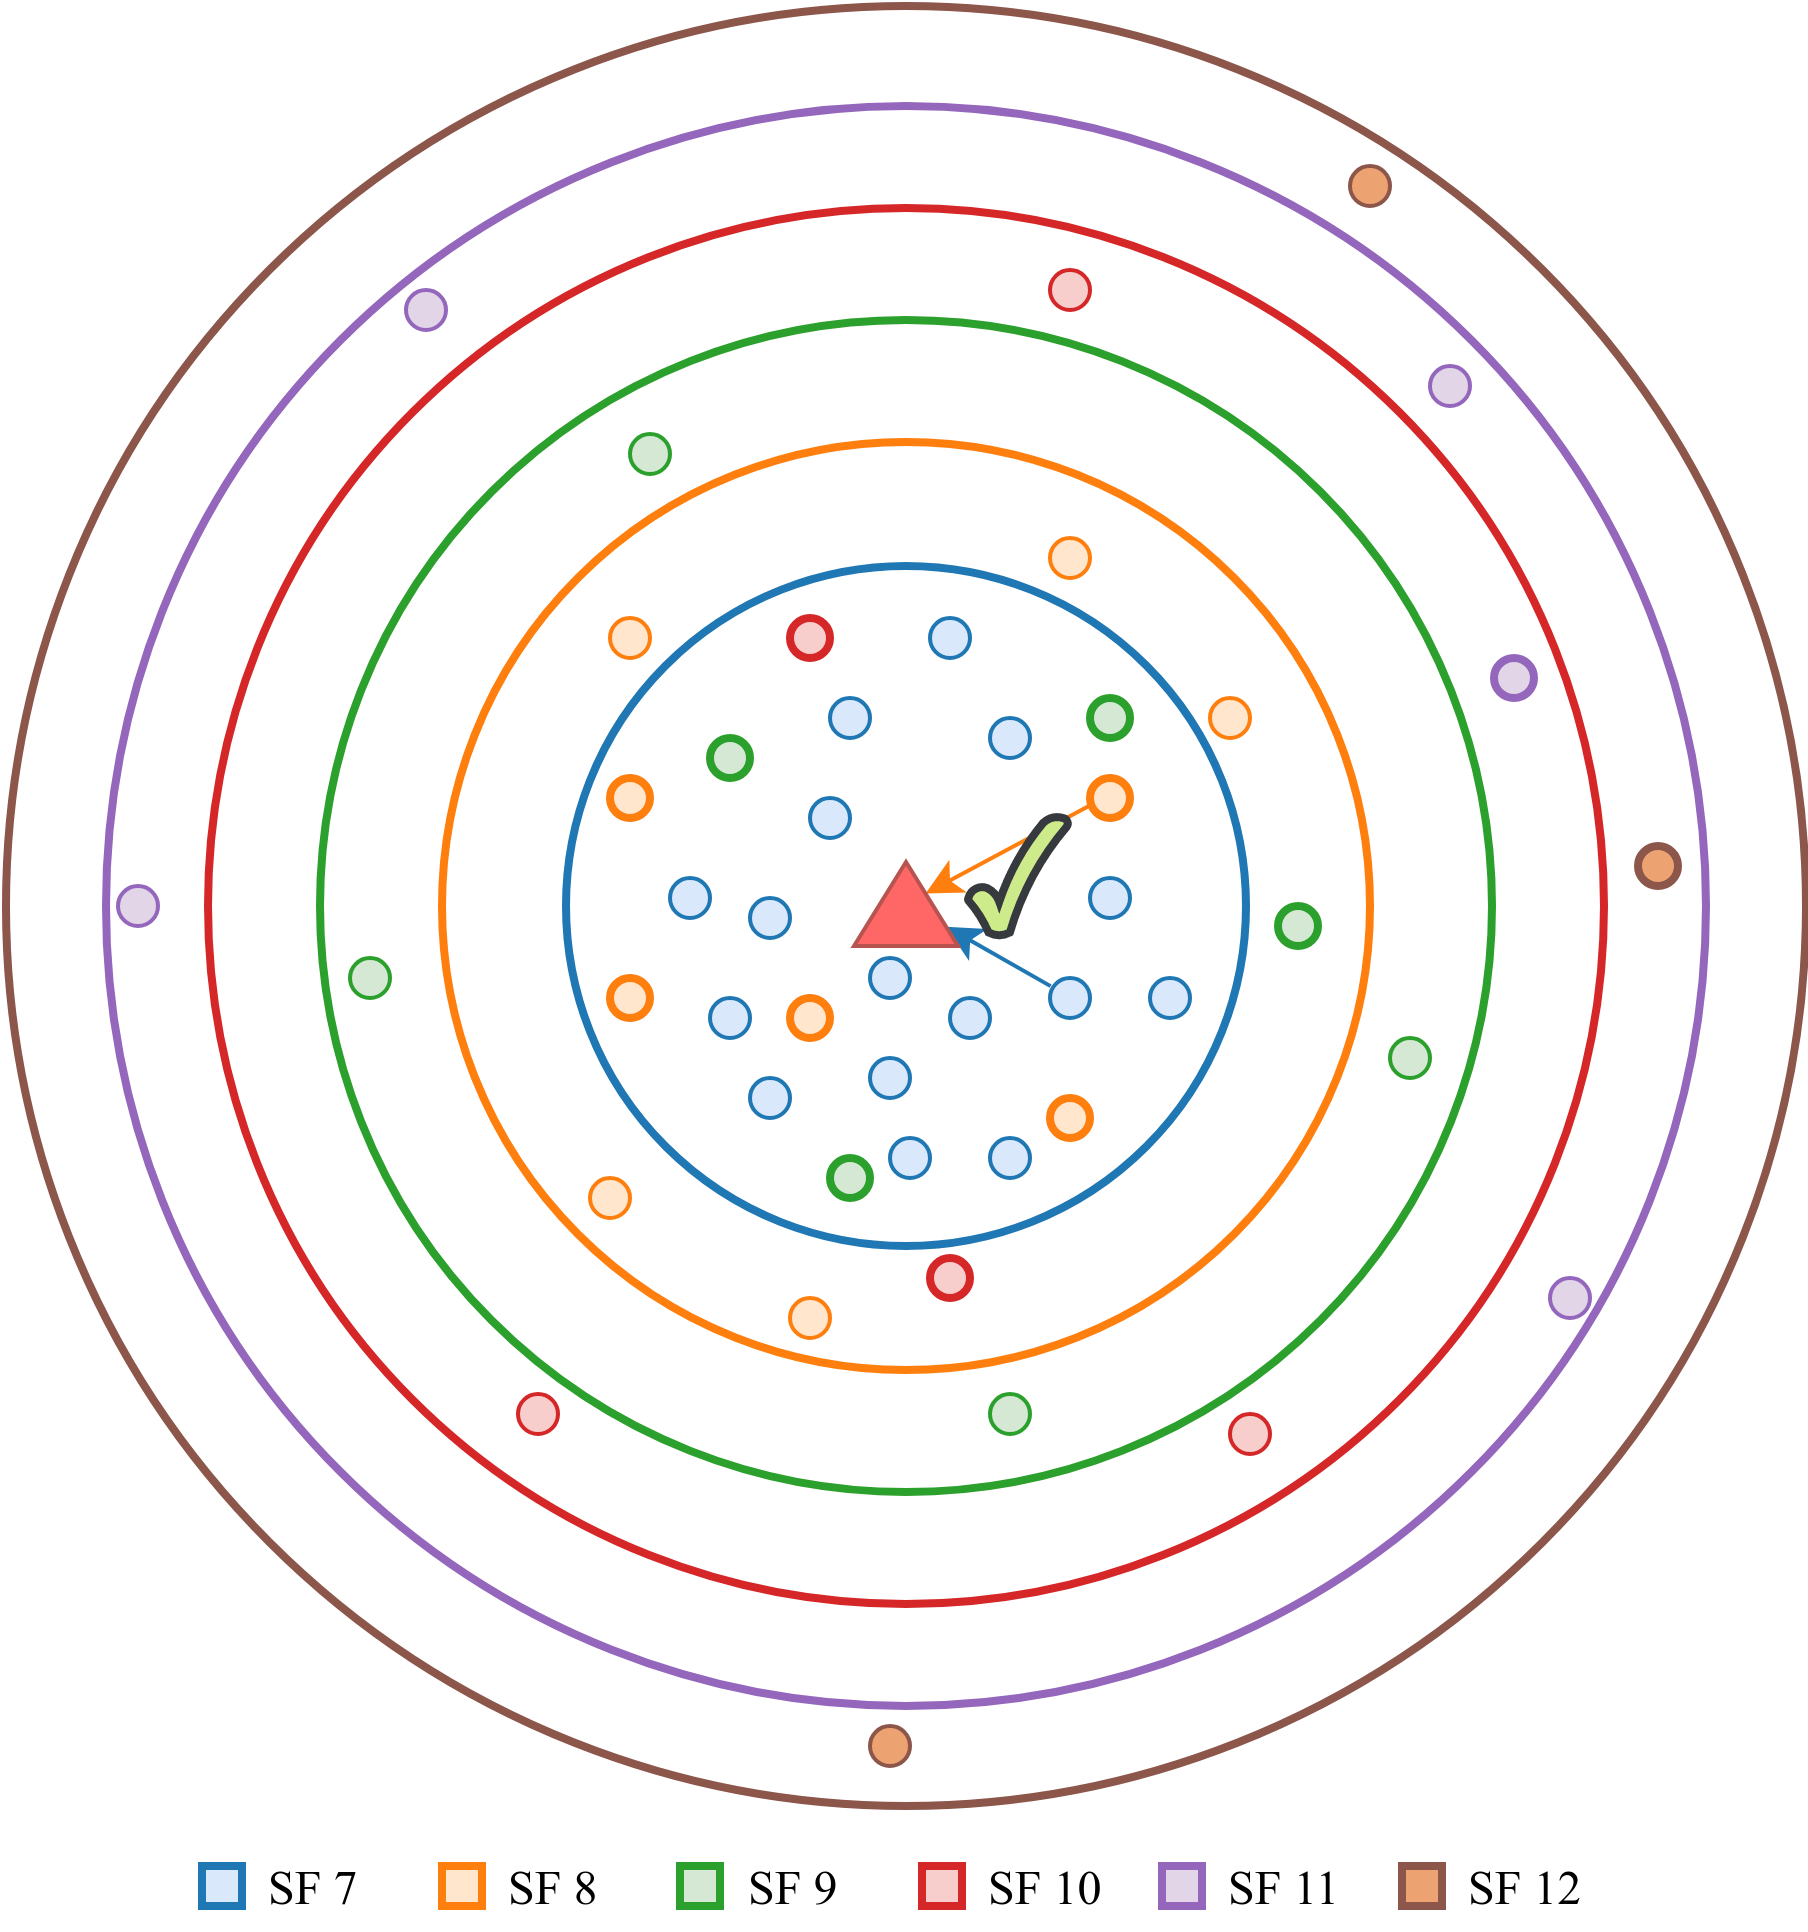
\includegraphics[width=0.85\linewidth]{collision_solution_single_gw.png}
\caption{Collision avoidance by using higher SF for nodes close to the gateway.}
\label{fig:collision_solution_single_gw}
\end{figure}

\begin{figure}
\centering
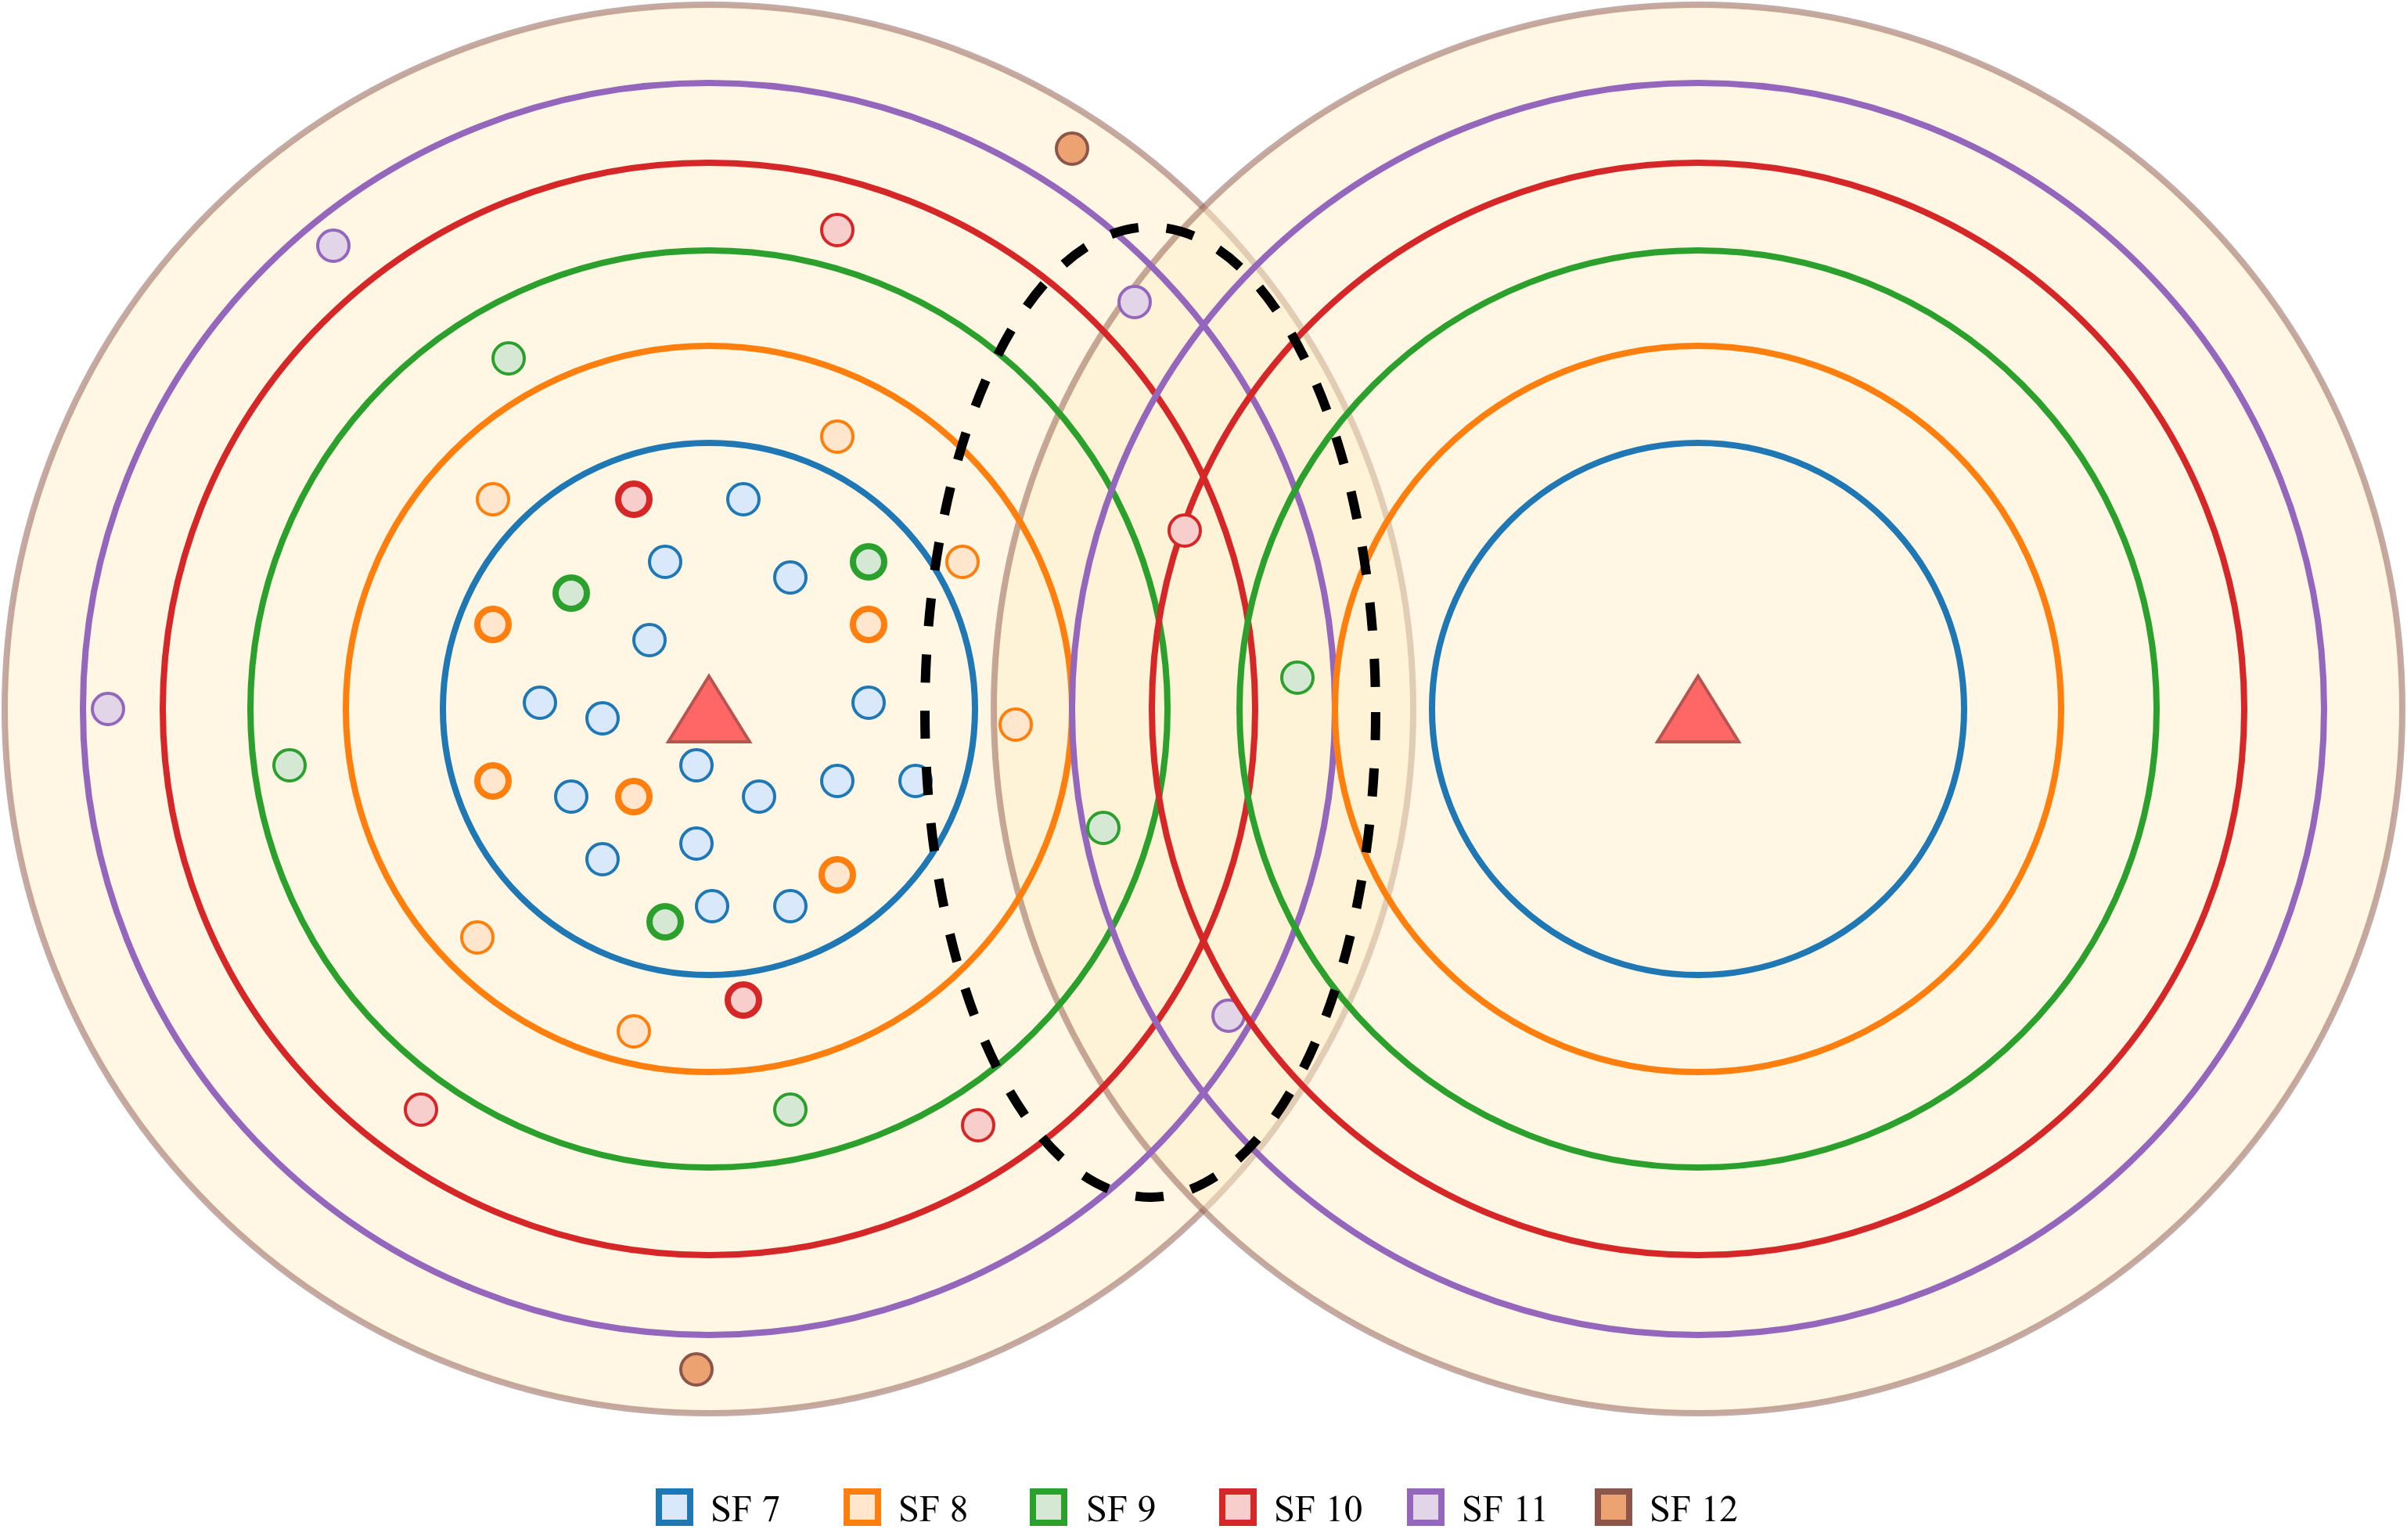
\includegraphics[width=\linewidth]{collision_solution_multi_gw.png}
\caption{Collision avoidance for intersecting gateways.}
\label{fig:collision_solution_multi_gw}
\end{figure}


\section{Simulation Environment} \label{Simulation Environment}
A discrete event simulator is developed in Python to study the effects of different SF strategies in LoRaWANs. LoRaWAN SF simulation tool source code is available at GitHub \cite{tugrul_yatagan_2019_2579366}. Simulation tool supports custom LoRaWAN topologies as well as randomly generated LoRaWAN topologies. Simulator can generate uniformly distributed circular shape network topology with following input parameters: radius (r) in meter (m), number of nodes and number of gateways. Global simulation input parameters are simulation duration in second (s), packet size in Byte (B), packet generation rate in packets per second (pps) and SF assignment method. With these inputs, the simulator produces total number of generated packets, number of successfully received packets, number of interfered packets, number of under sensitivity packets, network packet delivery ratio percentage (PDR), network throughput in bits per second (bps) and total transmit energy consumption in Joule (J). Simulator also produces prediction accuracy percentage and confusion matrix for machine learning schemes.

The simulator only covers the LoRaWAN Class A devices. Transmissions are always initiated by end nodes in pure ALOHA manner. Nodes generate a new packet randomly according to a Poisson interval for given packet rate parameter. Downlink transmissions are not considered. Downlink transmissions are rare in real world deployments since ISM band regulations dictate duty cycle transmission limit for all devices including gateways.

\subsection{Link Model Employed}
Link quality of a wireless system can be expressed by the metric of link budget. Link budget is a measure of all gains and losses from transmitter device to receiver device. Link budget of a wireless link can be calculated as \cite{AN1200.22}:

\begin{equation} \label{eq:expected_rx_power}
P^{dBm}_{RX} = P^{dBm}_{TX} + G^{dB}_{SYS} - L^{dB}_{SYS} - L^{dB}_{PATH}
\end{equation}

Where, $P^{dBm}_{RX}$ is the expected receive power at the receiver. $P^{dBm}_{TX}$ is the transmit power of the transmitter. $G^{dB}_{SYS}$ is the system gains such as transmitter and receiver antenna gains. $L^{dB}_{SYS}$ is the system losses such as transmitter and receiver line, circuit, antenna losses. $L^{dB}_{PATH}$ is the propagation path loss between transmitter and receiver antennas in open space. In the simulator, it is assumed that sum of system gains $G^{dB}_{SYS}$ and system losses $L^{dB}_{SYS}$ is +7 dB.

\begin{table}
\centering
\caption{EU863-870 ISM band LoRa default channels \cite{lorawan.regional.parameters}.}
\label{table:max_tx_power}
\begin{tabular}{|c|c|c|}
\hline
\textbf{Frequency (MHz)} & \textbf{Bandwidth (kHz)} & \textbf{Max EIRP (dBm)} \\ \hline
      868.1 &   125 &   14 \\ \hline
      868.3 &   125 &   14 \\ \hline
      868.5 &   125 &   14 \\ \hline
\end{tabular}
\end{table}

Maximum transmit power for European ISM band LoRa default channels can be found in Table \ref{table:max_tx_power}. In the simulator, it is assumed that nodes always select maximum allowed transmit power, which is 14 dBm. Different channel transmissions are independent from each other. But, in this work we focus on SF orthogonality. Thus, only single channel transmissions are utilized in the simulator.

\begin{table}
\centering
\caption{Gateway sensitivity for different SFs \cite{SX1276}.}
\label{table:gw_sf_sensitivity}
\begin{tabular}{|c|c|c|c|c|c|c|c|}
\hline
\multicolumn{2}{|c|}{\multirow{2}{*}{}} & \multicolumn{6}{c|}{\textbf{SF}} \\ \cline{3-8}
\multicolumn{2}{|c|}{}                  &    7 &    8 &    9 &   10 &   11 &   12 \\ \hline
\multirow{3}{*}{\textbf{BW (kHz)}}  & 125 & -123 & -126 & -129 & -132 & -133 & -136 \\ \cline{2-8}
                                    & 250 & -120 & -123 & -125 & -128 & -130 & -133 \\ \cline{2-8}
                                    & 500 & -116 & -119 & -122 & -125 & -128 & -130 \\ \hline
\end{tabular}
\end{table}

Receive sensitivity of a LoRa gateway for different SFs and BWs in dBm unit can be found in Table \ref{table:gw_sf_sensitivity}. In the simulator, 125 kHz bandwidth receive sensitivities are used.

Free space propagation loss is calculated as \cite{TR136.942}:

\begin{equation} \label{eq:propagation_loss}
\begin{split}
P^{dB}_{PATH} = 40(1 - 4 \times 10^{-3} \times h){\log_{10} R|_{km}} \\
- 18 {\log_{10} h|_{m}} + 21 {\log_{10} f|_{MHz}} + 80
\end{split}
\end{equation}

Where, $h$ is the gateway altitude and $f$ is the frequency of the signal. In this work, it is assumed that $h$ = 15 m and $f$ = 868 MHz. With these assumptions, propagation loss calculation become \cite{7996384}:

\begin{equation} \label{eq:propagation_loss_simplified}
P^{dB}_{PATH} = 120.5 + 37.6 {\log_{10} R|_{km}}
\end{equation}

If the received signal power is higher than the gateway sensitivity, then signal can be decoded by the receiver successfully when there is no interfering transmission.

\subsection{Interference Model Employed}
In the simulator, interference model described in \cite{7996384} is adopted. They use SINR threshold matrix for modeling LoRa interference between simultaneous but different SF LoRa transmissions.

In this work, it is assumed that there is no other technology interference in the network except LoRa interference. To exploit imperfect orthogonality of different SF transmission, simulator should calculate the effect of different SF transmissions to each other. In simulator, signal to interference plus noise ratio (SINR) threshold matrix $T_{i,j}$ from \cite{goursaud:hal-01231221} is used.

To decide if a referenced signal is interfered at receiver by an interfering signal, SINR threshold matrix is used. $T_{i,j}$ is SINR margin in dB unit between referenced signal with SF = i and interfering signal with SF = j to correctly decode the referenced signal. If there are more than one interfering signal, referenced signal must satisfy the margin for cumulative sum of all interfering signal received power for each SF \cite{7996384}. SINR threshold can be calculated as:

\begin{equation} \label{eq:sinr_db}
SINR_{i,j} = \dfrac{P_{rc,0}}{\sum_{l \in I_j} P_{rc,l}}
\end{equation}

Where $P_{rc,0}$ is received signal power of referenced signal and $P_{rc,l}$ is received signal power of interfering signal for SF = j. If a packet with SF = i satisfies the following condition for every SF = j, then packet is survived from all interferences.

\begin{equation} \label{eq:sinr_t}
SINR_{i,j}^{dB} > T_{i,j}
\end{equation}

To calculate interfering power at receiver, we should consider the case where two transmissions are not perfectly overlapping. To equalize the interfering power at receiver \cite{7996384}:

\begin{equation} \label{eq:p_interference}
P_{rc,y}^{interf} = \dfrac{P_{rc,y}(t_{interf})}{t_{x}}
\end{equation}

Where $t_{x}$ is transmission duration of referenced signal. $t_{interf}$ is overlapping duration between referenced signal and interfering signal. Transmission duration of a packet can be calculated by data rate $R_{b}$ and packet size $PS$. Data rate of a LoRa transmission is already expressed in Equation \ref{eq:bit_rate_sf}. Duration of a LoRa transmission can be calculated as:

\begin{equation} \label{eq:transmission_duration}
t_{x} = \dfrac{8 \times PS|_{B}}{R_{b}|_{bps}}  \ s
\end{equation}


\section{Simulation Results} \label{Simulation Results}
For simulation results in this paper, global simulation parameters are set as follows: packet size = 60 Bytes, simulation duration = 3600 seconds and packet generation rate = 0.01 pps. First, single gateway and multiple gateway LoRaWAN network simulation results are presented to show correctness of the simulator, then, smart SF scheme simulation results are presented.

\subsection{Single Gateway}
In Figure \ref{fig:sf_pdr}, PDR plots of various SF assignment schemes are shown. Randomly generated network topology radius is set to 3000 meters and number of gateways is set to 1. Increasing SFs increases air time. This increases the number of collisions thus decreases the PDR. High SF schemes gives poor PDR results as the number of nodes increases. Since network topology radius is quite small, all SFs can reach to gateway.

\begin{figure}
\centering
\includegraphics[width=\linewidth]{{sf_pdr_r3000_g1_p0.01_s3600}.png}
\caption{PDR for various SFs. (r = 3000 m, GW = 1)}
\label{fig:sf_pdr}
\end{figure}

In Figure \ref{fig:r_pdr}, PDR plots of various network radii are shown. Number of gateways is set to 1 and lowest SF assignment scheme is used. Increasing network radius, increases the number of under sensitivity transmissions thus decreases the PDR of network.

\begin{figure}
\centering
\includegraphics[width=\linewidth]{{r_pdr_g1_p0.01_s3600}.png}
\caption{PDR for various network radii. (GW = 1, SF = SF{\_}Lowest)}
\label{fig:r_pdr}
\end{figure}

\subsection{Multiple Gateway}
In Figure \ref{fig:gw_pdr}, PDR plots for various number of gateways are shown. Randomly generated topology radius is set to 3000 meters and the lowest SF assignment scheme is used. Increasing number of gateways, decreases the SFs of nodes and decreases air time. This decreases number of collisions, hence, increases the PDR of network when network radius is constant.

\begin{figure}
\centering
\includegraphics[width=\linewidth]{{gw_pdr_r3000_p0.01_s3600}.png}
\caption{PDR for various number of GWs. (r = 3000 m, SF = SF{\_}Lowest)}
\label{fig:gw_pdr}
\end{figure}

\subsection{Smart SF Schemes}
PDR plots of the lowest SF, random SF and the smart prediction schemes are shown in Figure \ref{fig:prediction_pdr}. Randomly generated network radius is set to 5000 meters and number of gateways is set to 3. Prediction model needs nodes' locations and three gateways are enough to locate position of nodes by triangulation. In Table \ref{table:prediction_pdr}, PDR values for various network radii are presented. Both smart SVM and smart DTC schemes give better PDR than lowest SF schemes when number of nodes increases. Increasing number of nodes, increases number of interferences. Smart schemes improve network performance when LoRa interference is high. Moreover, smart schemes give better results when nodes are deployed closer to the gateway, since nodes have margin to increase their SFs when they are deployed closer to the gateway. If a node is far away from gateway, then smart schemes cannot increase the SF to avoid interference since the assigned SF is already high.

In Table \ref{table:prediction_accuracy}, prediction accuracy of smart SVM and smart DTC schemes are presented for various network radii and number of nodes. Prediction accuracy is not directly proportional to network PDR. Correct prediction of an interfered transmission may not increase the PDR but increases the prediction accuracy. Smart DTC gives better network PDR results than smart SVM, even overall smart SVM prediction accuracy is higher. The distribution of different labeled data points in the dataset is strongly related to simulation parameters. If simulation is run with small topology radius and high number of nodes, then number of interfered transmission labeled data points increases. On the other hand, using a large topology radius in the simulation causes the number of under sensitivity transmission labeled data points to increase. We choose moderately dense network parameters to bring it closer to real world deployments. With the simulation parameters utilized in this section, simulation usually produces imbalanced dataset. Number of under sensitivity transmission labeled data points are less than number of successful transmission labeled data points. Besides, number of interfered transmission labeled data points are even less then number of under sensitivity transmission labeled data points. In this case, smart DTC predicts interfered transmission labeled data points more accurately. Correct classification of interfered transmissions yields better network PDR results, thus smart DTC scheme gives better network PDR results.

\begin{figure}
\centering
\includegraphics[width=\linewidth]{{prediction_pdr_r5000_g3_p0.01_s3600}.png}
\caption{PDR for lowest and smart SF schemes. (r = 5000 m, GW = 3)}
\label{fig:prediction_pdr}
\end{figure}

\begin{table}
\centering
\caption{PDR for lowest and smart SF schemes. (GW = 3)}
\label{table:prediction_pdr}
\begin{tabular}{|c|c|c|c|c|c|}
\hline
\multicolumn{3}{|c|}{\multirow{2}{*}{}}                            & \multicolumn{3}{c|}{\textbf{Number of Nodes}} \\ \cline{4-6}
\multicolumn{3}{|c|}{}                                             & 100           & 500           & 1000          \\ \hline
\multirow{12}{*}{\textbf{r (m)}} & \multirow{3}{*}{3000}  & Lowest & 97.8          & 86.0          & 72.3          \\ \cline{3-6}
                                 &                        & SVM    & 98.0          & 88.2          & 75.2          \\ \cline{3-6}
                                 &                        & DTC    & 97.8          & 89.8          & 78.7          \\ \cline{2-6}

                                 & \multirow{3}{*}{5000}  & Lowest & 96.8          & 85.5          & 71.2          \\ \cline{3-6}
                                 &                        & SVM    & 98.0          & 87.8          & 74.8          \\ \cline{3-6}
                                 &                        & DTC    & 97.7          & 90.2          & 79.8          \\ \cline{2-6}

                                 & \multirow{3}{*}{7000}  & Lowest & 97.2          & 87.5          & 76.8          \\ \cline{3-6}
                                 &                        & SVM    & 98.2          & 88.8          & 78.6          \\ \cline{3-6}
                                 &                        & DTC    & 97.8          & 90.7          & 81.6          \\ \cline{2-6}

                                 & \multirow{3}{*}{10000} & Lowest & 98.2          & 90.3          & 81.5          \\ \cline{3-6}
                                 &                        & SVM    & 98.3          & 90.3          & 81.9          \\ \cline{3-6}
                                 &                        & DTC    & 98.3          & 90.6          & 81.9          \\ \hline
\end{tabular}
\end{table}

\begin{table}
\centering
\caption{Prediction accuracy for SVM and DTC. (GW = 3)}
\label{table:prediction_accuracy}
\begin{tabular}{|c|c|c|c|c|c|}
\hline
\multicolumn{3}{|c|}{\multirow{2}{*}{}}                        & \multicolumn{3}{c|}{\textbf{Number of Nodes}} \\ \cline{4-6}
\multicolumn{3}{|c|}{}                                         & 100           & 500           & 1000          \\ \hline
\multirow{8}{*}{\textbf{r (m)}} & \multirow{2}{*}{3000}  & SVM & 82.4          & 70.4          & 71.7          \\ \cline{3-6}
                                &                        & DTC & 86.0          & 67.3          & 70.4          \\ \cline{2-6}

                                & \multirow{2}{*}{5000}  & SVM & 79.5          & 69.0          & 71.1          \\ \cline{3-6}
                                &                        & DTC & 84.5          & 67.3          & 69.5          \\ \cline{2-6}

                                & \multirow{2}{*}{7000}  & SVM & 79.5          & 70.6          & 71.2          \\ \cline{3-6}
                                &                        & DTC & 84.5          & 67.7          & 69.2          \\ \cline{2-6}

                                & \multirow{2}{*}{10000} & SVM & 79.2          & 74.4          & 76.1          \\ \cline{3-6}
                                &                        & DTC & 83.8          & 70.7          & 74.3          \\ \hline
\end{tabular}
\end{table}

For space constraints, we omit simulation results like network throughput, total transmit energy consumption and confusion matrices. We invite readers to experiment the simulation tool with the parameters they like \cite{tugrul_yatagan_2019_2579366}.


\section{Conclusion} \label{Conclusion}
In this paper, after a brief introduction about LPWAN technologies, LoRa modulation basics and spreading factor assignment issue is discussed. We present an open source discrete event simulator which is developed from scratch to study network performance of LoRaWAN and evaluate different SF assignment schemes. Moreover, we show how same SF collisions can be avoided, hence, we propose a machine learning based solutions called smart DTC scheme and smart SVM scheme. We present simulation results for the lowest SF assignment scheme and the proposed schemes. Simulation results show that, the proposed smart schemes can increase network performance for LoRaWAN networks, especially, when the nodes are deployed close to gateways.

As for future work, transmit power optimization can be included to the proposed smart scheme. In this paper, it is assumed that nodes always use maximum transmit power for uplink transmission, however nodes close to gateways can decrease transmit power to save energy. This will make transmissions more vulnerable to interference thus requires extra care. Moreover, other machine learning methods can be investigated for SF assignment enhancement. Reinforcement learning could be a good candidate. Also, other transmission parameters such as node id and transmission time can be included to the proposed scheme in order to improve prediction performance.


\section*{Acknowledgment}
This work is supported by Turkish Ministry of Development and Istanbul Technical University researcher support program under the Grant No. ITU-AYP-2017-1.


\bibliographystyle{IEEEtran}
\bibliography{references}

\end{document}
